\definecolor{colorPortada}{RGB}{240,240,110}
\pagecolor{colorPortada}

\addcontentsline{toc}{chapter}{Portada}

\begin{titlepage}
   \parbox{18cm}{\fontsize{60pt}{60pt}\selectfont\color{red}\scshape%
                 Qüestions\\[25pt] Electrotècniques\\[25pt] Diverses\\[80pt]%
                 \fontsize{40pt}{40pt}\selectfont{}Josep Mollera Barriga}
   \vspace*{10mm}
   \begin{center}
        \fontsize{10pt}{11pt}\selectfont
        % GNUPLOT: LaTeX picture with Postscript
\begingroup
  \makeatletter
  \providecommand\color[2][]{%
    \GenericError{(gnuplot) \space\space\space\@spaces}{%
      Package color not loaded in conjunction with
      terminal option `colourtext'%
    }{See the gnuplot documentation for explanation.%
    }{Either use 'blacktext' in gnuplot or load the package
      color.sty in LaTeX.}%
    \renewcommand\color[2][]{}%
  }%
  \providecommand\includegraphics[2][]{%
    \GenericError{(gnuplot) \space\space\space\@spaces}{%
      Package graphicx or graphics not loaded%
    }{See the gnuplot documentation for explanation.%
    }{The gnuplot epslatex terminal needs graphicx.sty or graphics.sty.}%
    \renewcommand\includegraphics[2][]{}%
  }%
  \providecommand\rotatebox[2]{#2}%
  \@ifundefined{ifGPcolor}{%
    \newif\ifGPcolor
    \GPcolortrue
  }{}%
  \@ifundefined{ifGPblacktext}{%
    \newif\ifGPblacktext
    \GPblacktexttrue
  }{}%
  % define a \g@addto@macro without @ in the name:
  \let\gplgaddtomacro\g@addto@macro
  % define empty templates for all commands taking text:
  \gdef\gplbacktext{}%
  \gdef\gplfronttext{}%
  \makeatother
  \ifGPblacktext
    % no textcolor at all
    \def\colorrgb#1{}%
    \def\colorgray#1{}%
  \else
    % gray or color?
    \ifGPcolor
      \def\colorrgb#1{\color[rgb]{#1}}%
      \def\colorgray#1{\color[gray]{#1}}%
      \expandafter\def\csname LTw\endcsname{\color{white}}%
      \expandafter\def\csname LTb\endcsname{\color{black}}%
      \expandafter\def\csname LTa\endcsname{\color{black}}%
      \expandafter\def\csname LT0\endcsname{\color[rgb]{1,0,0}}%
      \expandafter\def\csname LT1\endcsname{\color[rgb]{0,1,0}}%
      \expandafter\def\csname LT2\endcsname{\color[rgb]{0,0,1}}%
      \expandafter\def\csname LT3\endcsname{\color[rgb]{1,0,1}}%
      \expandafter\def\csname LT4\endcsname{\color[rgb]{0,1,1}}%
      \expandafter\def\csname LT5\endcsname{\color[rgb]{1,1,0}}%
      \expandafter\def\csname LT6\endcsname{\color[rgb]{0,0,0}}%
      \expandafter\def\csname LT7\endcsname{\color[rgb]{1,0.3,0}}%
      \expandafter\def\csname LT8\endcsname{\color[rgb]{0.5,0.5,0.5}}%
    \else
      % gray
      \def\colorrgb#1{\color{black}}%
      \def\colorgray#1{\color[gray]{#1}}%
      \expandafter\def\csname LTw\endcsname{\color{white}}%
      \expandafter\def\csname LTb\endcsname{\color{black}}%
      \expandafter\def\csname LTa\endcsname{\color{black}}%
      \expandafter\def\csname LT0\endcsname{\color{black}}%
      \expandafter\def\csname LT1\endcsname{\color{black}}%
      \expandafter\def\csname LT2\endcsname{\color{black}}%
      \expandafter\def\csname LT3\endcsname{\color{black}}%
      \expandafter\def\csname LT4\endcsname{\color{black}}%
      \expandafter\def\csname LT5\endcsname{\color{black}}%
      \expandafter\def\csname LT6\endcsname{\color{black}}%
      \expandafter\def\csname LT7\endcsname{\color{black}}%
      \expandafter\def\csname LT8\endcsname{\color{black}}%
    \fi
  \fi
    \setlength{\unitlength}{0.0500bp}%
    \ifx\gptboxheight\undefined%
      \newlength{\gptboxheight}%
      \newlength{\gptboxwidth}%
      \newsavebox{\gptboxtext}%
    \fi%
    \setlength{\fboxrule}{0.5pt}%
    \setlength{\fboxsep}{1pt}%
\begin{picture}(9340.00,5660.00)%
    \gplgaddtomacro\gplbacktext{%
      \colorrgb{0.00,0.00,0.00}%%
      \put(752,787){\makebox(0,0)[r]{\strut{} 0}}%
      \colorrgb{0.00,0.00,0.00}%%
      \put(752,1097){\makebox(0,0)[r]{\strut{} 10}}%
      \colorrgb{0.00,0.00,0.00}%%
      \put(752,1407){\makebox(0,0)[r]{\strut{} 20}}%
      \colorrgb{0.00,0.00,0.00}%%
      \put(752,1718){\makebox(0,0)[r]{\strut{} 30}}%
      \colorrgb{0.00,0.00,0.00}%%
      \put(752,2028){\makebox(0,0)[r]{\strut{} 40}}%
      \colorrgb{0.00,0.00,0.00}%%
      \put(752,2338){\makebox(0,0)[r]{\strut{} 50}}%
      \colorrgb{0.00,0.00,0.00}%%
      \put(752,2648){\makebox(0,0)[r]{\strut{} 60}}%
      \colorrgb{0.00,0.00,0.00}%%
      \put(752,2958){\makebox(0,0)[r]{\strut{} 70}}%
      \colorrgb{0.00,0.00,0.00}%%
      \put(752,3269){\makebox(0,0)[r]{\strut{} 80}}%
      \colorrgb{0.00,0.00,0.00}%%
      \put(752,3579){\makebox(0,0)[r]{\strut{} 90}}%
      \colorrgb{0.00,0.00,0.00}%%
      \put(752,3889){\makebox(0,0)[r]{\strut{} 100}}%
      \colorrgb{0.00,0.00,0.00}%%
      \put(752,4199){\makebox(0,0)[r]{\strut{} 110}}%
      \colorrgb{0.00,0.00,0.00}%%
      \put(752,4509){\makebox(0,0)[r]{\strut{} 120}}%
      \colorrgb{0.00,0.00,0.00}%%
      \put(752,4820){\makebox(0,0)[r]{\strut{} 130}}%
      \colorrgb{0.00,0.00,0.00}%%
      \put(752,5130){\makebox(0,0)[r]{\strut{} 140}}%
      \colorrgb{0.00,0.00,0.00}%%
      \put(752,5440){\makebox(0,0)[r]{\strut{} 150}}%
      \colorrgb{0.00,0.00,0.00}%%
      \put(936,481){\makebox(0,0){\strut{} 0}}%
      \colorrgb{0.00,0.00,0.00}%%
      \put(1424,481){\makebox(0,0){\strut{} 100}}%
      \colorrgb{0.00,0.00,0.00}%%
      \put(1912,481){\makebox(0,0){\strut{} 200}}%
      \colorrgb{0.00,0.00,0.00}%%
      \put(2400,481){\makebox(0,0){\strut{} 300}}%
      \colorrgb{0.00,0.00,0.00}%%
      \put(2888,481){\makebox(0,0){\strut{} 400}}%
      \colorrgb{0.00,0.00,0.00}%%
      \put(3376,481){\makebox(0,0){\strut{} 500}}%
      \colorrgb{0.00,0.00,0.00}%%
      \put(3864,481){\makebox(0,0){\strut{} 600}}%
      \colorrgb{0.00,0.00,0.00}%%
      \put(4352,481){\makebox(0,0){\strut{} 700}}%
      \colorrgb{0.00,0.00,0.00}%%
      \put(4841,481){\makebox(0,0){\strut{} 800}}%
      \colorrgb{0.00,0.00,0.00}%%
      \put(5329,481){\makebox(0,0){\strut{} 900}}%
      \colorrgb{0.00,0.00,0.00}%%
      \put(5817,481){\makebox(0,0){\strut{} 1000}}%
      \colorrgb{0.00,0.00,0.00}%%
      \put(6305,481){\makebox(0,0){\strut{} 1100}}%
      \colorrgb{0.00,0.00,0.00}%%
      \put(6793,481){\makebox(0,0){\strut{} 1200}}%
      \colorrgb{0.00,0.00,0.00}%%
      \put(7281,481){\makebox(0,0){\strut{} 1300}}%
      \colorrgb{0.00,0.00,0.00}%%
      \put(7769,481){\makebox(0,0){\strut{} 1400}}%
      \colorrgb{0.00,0.00,0.00}%%
      \put(8257,481){\makebox(0,0){\strut{} 1500}}%
      \colorrgb{0.00,0.00,0.00}%%
      \put(8441,787){\makebox(0,0)[l]{\strut{} 0}}%
      \colorrgb{0.00,0.00,0.00}%%
      \put(8441,1097){\makebox(0,0)[l]{\strut{} 5}}%
      \colorrgb{0.00,0.00,0.00}%%
      \put(8441,1407){\makebox(0,0)[l]{\strut{} 10}}%
      \colorrgb{0.00,0.00,0.00}%%
      \put(8441,1718){\makebox(0,0)[l]{\strut{} 15}}%
      \colorrgb{0.00,0.00,0.00}%%
      \put(8441,2028){\makebox(0,0)[l]{\strut{} 20}}%
      \colorrgb{0.00,0.00,0.00}%%
      \put(8441,2338){\makebox(0,0)[l]{\strut{} 25}}%
      \colorrgb{0.00,0.00,0.00}%%
      \put(8441,2648){\makebox(0,0)[l]{\strut{} 30}}%
      \colorrgb{0.00,0.00,0.00}%%
      \put(8441,2958){\makebox(0,0)[l]{\strut{} 35}}%
      \colorrgb{0.00,0.00,0.00}%%
      \put(8441,3269){\makebox(0,0)[l]{\strut{} 40}}%
      \colorrgb{0.00,0.00,0.00}%%
      \put(8441,3579){\makebox(0,0)[l]{\strut{} 45}}%
      \colorrgb{0.00,0.00,0.00}%%
      \put(8441,3889){\makebox(0,0)[l]{\strut{} 50}}%
      \colorrgb{0.00,0.00,0.00}%%
      \put(8441,4199){\makebox(0,0)[l]{\strut{} 55}}%
      \colorrgb{0.00,0.00,0.00}%%
      \put(8441,4509){\makebox(0,0)[l]{\strut{} 60}}%
      \colorrgb{0.00,0.00,0.00}%%
      \put(8441,4820){\makebox(0,0)[l]{\strut{} 65}}%
      \colorrgb{0.00,0.00,0.00}%%
      \put(8441,5130){\makebox(0,0)[l]{\strut{} 70}}%
      \colorrgb{0.00,0.00,0.00}%%
      \put(8441,5440){\makebox(0,0)[l]{\strut{} 75}}%
    }%
    \gplgaddtomacro\gplfronttext{%
      \csname LTb\endcsname%%
      \put(255,3113){\rotatebox{-270}{\makebox(0,0){\strut{}$T\ped{m}\, / \,\si{N.m}$}}}%
      \csname LTb\endcsname%%
      \put(8938,3113){\rotatebox{-270}{\makebox(0,0){\strut{}$I_1\, / \,\si{A}$}}}%
      \csname LTb\endcsname%%
      \put(4596,153){\makebox(0,0){\strut{}$n\ped{m}\, / \,\si{r/min}$}}%
      \csname LTb\endcsname%%
      \put(4596,5331){\makebox(0,0){\strut{}}}%
      \csname LTb\endcsname%%
      \put(4596,5440){\makebox(0,0){\strut{}}}%
      \csname LTb\endcsname%%
      \put(1440,1530){\makebox(0,0){\strut{}}}%
      \csname LTb\endcsname%%
      \put(1508,1448){\makebox(0,0)[l]{\strut{}$T\ped{m}$}}%
      \csname LTb\endcsname%%
      \put(1508,1120){\makebox(0,0)[l]{\strut{}$I_1$}}%
      \csname LTb\endcsname%%
      \put(2400,2763){\makebox(0,0){$\scriptstyle\SI{60,7}{N.m}$}}%
      \csname LTb\endcsname%%
      \put(2400,4996){\makebox(0,0){$\scriptstyle\SI{132,7}{N.m}$}}%
      \csname LTb\endcsname%%
      \put(7808,1407){\rotatebox{-270}{\makebox(0,0){$\scriptstyle\SI{1425}{r/min}$}}}%
      \csname LTb\endcsname%%
      \put(6500,1469){\rotatebox{-270}{\makebox(0,0){$\scriptstyle\SI{1157,6}{r/min}$}}}%
    }%
    \gplbacktext
    \put(0,0){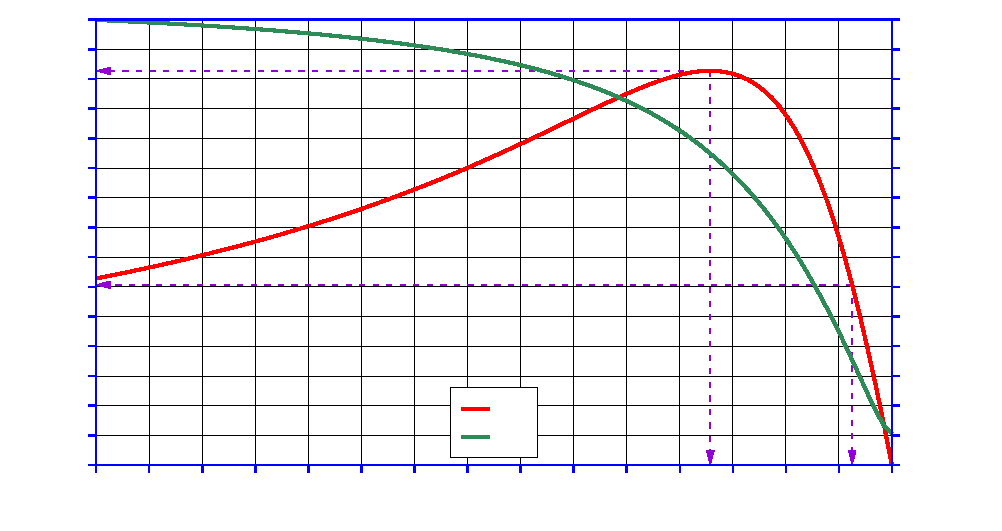
\includegraphics{Cap-Motors-Induccio-Ex4}}%
    \gplfronttext
  \end{picture}%
\endgroup

   \end{center}
\end{titlepage}

\pagecolor{white}

\cleardoublepage\thispagestyle{empty}
\phantomsection\addcontentsline{toc}{chapter}{Copyright}
{\fontsize{60pt}{60pt}\selectfont%
Qüestions\\[25pt]
Electrotècniques\\[25pt]
Diverses\\[90pt]}
{\fontsize{40pt}{40pt}\selectfont
2005-2019 \hspace{5mm}{\Huge(versió 11.2)}\\[85pt]
Josep Mollera Barriga\\[25pt]}
{\fontsize{25pt}{25pt}\selectfont
Enginyer Industrial per l'ETSEIB (UPC)}
\vfill
{\fontsize{15pt}{20pt}\selectfont
\begin{list}{}
    {\setlength{\labelwidth}{7mm} \setlength{\leftmargin}{7mm}\setlength{\labelsep}{2mm}}
    \item[\faCopyright]  Qualsevol part d'aquest llibre  pot  distribuir-se lliurament
                         sempre que se’n reconegui l’autoria i no se’n faci un ús comercial.
\end{list}}

\cleardoublepage\thispagestyle{empty}
\phantomsection\addcontentsline{toc}{chapter}{Citacions}
\vspace{10cm}\hspace{10cm}
\parbox{6cm}{If I have seen further it is by standing on the shoulders of Giants.\\[10pt]
\textbf{Isaac Newton}\\[40pt]
I never am really satisfied that I understand anything; because, understand it well as I may, my comprehension can only be an infinitesimal fraction of all I want to understand about the many connections and relations which occur to me.\\[10pt]
\textbf{Ada Lovelace}\\[40pt]
Dans la vie, rien n'est à craindre, tout est à comprendre.\\[10pt]
\textbf{Marie Curie}\\[40pt]
The first principle is that you must not fool yourself -- and you are the easiest person to fool.\\[10pt]
\textbf{Richard Feynman}\\[40pt]
I hope you will disdain mediocrity and aim to excel in whatever you do. I hope you will fight injustice and discrimination in all of its guises.\\[10pt]
\textbf{Vera Rubin}\\[40pt]
I would like people to appreciate science in the same way they appreciate the arts.\\[10pt]
\textbf{Richard Dawkins}}
